\chapter{The DFT approach} \label{ch:DFT}
As with the DFT the DCT have diagonalization properties for specific types of matrices. These properties will be presented in the context of convolution and boundary conditions. Recall when the kernel $k(x,t)$ is of the form $k(x,t) = k(x-t)$, \eqref{eq:FIE} is specific case of the convolution
\begin{equation}
\label{eq:Inf. Cont. Conv.}
g(x) = \int_{-\infty}^{\infty} k(x-t)f(t) ~dt.
\end{equation}
The functions $k$ and $f$ can be expressed as bi-infinite sequences by sampling the functions at a countable number of points in $\mathbb{R}$:
\[(k_n) = (\ldots,k_{-1},k_{0},k_{1},\ldots), \quad (f_n) = (\ldots,f_{-1},f_{0},f_{1},\ldots).\]
The convolution \eqref{eq:Inf. Cont. Conv.} then has an analogous definition for sequences; the $j$th entry $g_j$ of $(g_n)$ is
\begin{equation}
\label{eq:Inf. Disc. Conv.}
g_j = \sum_{\ell=-\infty}^{\infty} k_{j-\ell}f_{\ell}.
\end{equation}
If the kernel has compact support, then $(k_n)$ will have finitely many nonzero terms and can be expressed as
\begin{equation}
\label{eq:Kernel seq.}
(k_n) = (\ldots,0,k_{-m+1},\ldots,k_{-1},k_{0},k_{1},\ldots,k_{m-1},0,\ldots),
\end{equation}
In this representation $(k_n)$ has $2m-1$ nonzero terms. Furthermore if the data vector $\gnoiseVec$ has length $n$, then \eqref{eq:Inf. Disc. Conv.} can be expressed as the matrix-vector product
\begin{equation}
\label{eq:FIEv. Prod.}
\begin{bmatrix}
k_{m-1} & \cdots & k_0 & \cdots k_{-m+1} & & & & & \\
 & k_{m-1} & & k_0 & & k_{-m+1} & & & 0 & \\
 & & \ddots & \ddots & \ddots & \ddots & \ddots & & & \\
 & & & \ddots & \ddots & \ddots & \ddots & \ddots & & \\
 & 0 & & & k_{m-1} & & k_0 & & k_{-m+1} & \\
 & & & & & k_{m-1} & \cdots & k_0 & \cdots & k_{-m+1}
\end{bmatrix}\begin{bmatrix}
f_{-m+2} \\
f_{-m+3} \\
\vdots \\
f_0 \\
f_1 \\
\vdots \\
f_{n-1} \\
f_n \\
\vdots \\
f_{n+m-2} \\
f_{n+m-1}
\end{bmatrix}.
\end{equation}
The product \eqref{eq:FIEv. Prod.} can be expressed as
\begin{equation}
\label{eq: Tf = g}
T_{l}\fVec_{l} + T\fVec + T_{r}\fVec_{r} = \gVec
\end{equation}
where
\[\fVec_{l} = \begin{bmatrix}
f_{-m+2} \\
f_{-m+3} \\
\vdots \\
f_{-1}
\end{bmatrix}, \quad \fVec = \begin{bmatrix}
f_{0} \\
f_{1} \\
\vdots \\
f_{n-1}
\end{bmatrix}, \quad \fVec_{r} = \begin{bmatrix}
f_{n} \\
f_{n+1} \\
\vdots \\
f_{n+m-1}
\end{bmatrix}\]
and
\[T_{l} = \begin{bmatrix}
k_{m-1} & \cdots & k_{1} \\
 & \ddots & \ddots \\
 & & k_{m-1} \\
 & & \\
0 & & 
\end{bmatrix},
T = \begin{bmatrix}
k_{0} & \cdots & k_{-m+1} & & 0 \\
\vdots & \ddots & \ddots & \ddots &  \\
k_{m-1} & \ddots & \ddots & \ddots & k_{-m+1} \\
 & \ddots & \ddots & \ddots & \vdots \\
0 & & k_{m-1} & \cdots & k_{0} \\
\end{bmatrix}
T_{r} = \begin{bmatrix}
 & & 0 \\
 & & \\
k_{-m+1} & & \\
\vdots & \ddots &  \\
k_{-1} & \cdots & k_{-m+1} \\
\end{bmatrix}.\]
The goal is tto obtain a solution $\fVec = [f_0,\ldots,f_{n-1}]^\trans$. However, it is clear that $\fVec$ depends not only upon the choice of kernel $k$ but on the boundaries of $\fVec$, i.e. the terms $f_j$ of $(f_n)$ where $j \not\in \{0,1,n-1\}$. There are a number of ways in which the boundaries can be handled; Dirichlet, periodic, and Neumann boundary conditions are considered in \cite{NeumannDCT}. The most-simplifying condition in terms of the result system is the Dirichlet condition, which assumed that $\fVec_l = \fVec_r = \zeroVec$. The resulting system \eqref{eq: Tf = g} is $T\fVec = \gVec$. The matrix $T$ is Toeplitz, and methods such as those presented in \cite{Vogel:2002} can be used to obtain solutions. The situation becomes more complicated in higher dimensions: for 2D problems, the system matrix is block-Toeplitz with Toeplitz blocks and solving such a system requires $O(n^4)$ operations \cite{KalouptsidisCarayannisManolakis}. \par 
The DFT is well-suited for situations in which the boundary conditions are assumed to be periodic. For one-dimensional problem, the resulting kernel matrix $\kMat$ is circulant and is therefore diagonalized by the DFT. For two-dimensional problems, $\kMat$ is a block-circulant matrix with circulant blocks; adopting the notation from \cite[p.~71-72]{Vogel:2002}, such matrices will be referred to as BCCB matrices. Analogously, BCCB matrices can be diagonalized with two-dimensional DFTs. \par 
Focusing on the one-dimension case, imposing periodic boundary conditions on $\fVec$ means that $f_j = f_{n-j}$ in \eqref{eq:FIEv. Prod.} The result is that \eqref{eq: Tf = g} becomes
\[ C\fVec = [(\zeroVec ~|~ T_l) + T + (T_r ~|~ \zeroVec)]\fVec = \gVec,\]
where $C$ is a circulant matrix. The diagonalization property \eqref{eq:CircDiag} then allows for the Tikhonov regularization parameter to be determined by DFT-versions of the methods in Chapter \ref{ch:Parameter estimation methods}. 

%\section{Accuracy of the DFT components} \label{sec:Accuracy of DFT}
%
%As stated at the start of Chapter \ref{ch:DFT}, the DFT can be derived as an approximation of the Fourier coefficients of a given function. The relationships between the DFT and Fourier coefficients will now be discussed. \par 
%Let $\Pi$ denote the vector space of integrable complex-valued functions defined on $\mathbb{R}$ with period 1. We only consider function that are integrable real-valued and defined on $[0,1]$, though their periodic extensions are contained in $\Pi$.  The Fourier coefficients of a function $f \in \Pi$ are given by 
%\begin{equation}
%\label{eq:Fourier coefficients}
%c_j = \int_0^1 f(t)\exp(-2\pi{i}jt) \: dt, j \in \mathbb{Z}
%\end{equation}
%so that the $f$ can be expanded as the Fourier series
%\begin{equation}
%\label{eq:Fourier series}
%f(x) = \sum_{j=-\infty}^{\infty} c_j \exp(2\pi{i}jx).
%\end{equation}
%The expansion of functions as Fourier series relies on the fact that the set $\{\exp(2\pi{i}jx)\:|\:j\in\mathbb{Z}\}$ forms is an orthonormal basis for $\Pi$; the Fourier coefficients \eqref{eq:Fourier coefficients} are inner products of the function $f$ with these basis elements. \par
%Letting $\mathbf{f}$ be the $n$-point discretization of $f$ on $[0,1]$ defined by $f_j = f(j/n)$ with $j \in \{0,\ldots,n-1\}$, the difference between $c_j$ and $\dft{f}_j$ can be conveniently quantified if the Fourier series of $f$ is assumed to be absolutely convergent, i.e.
%\[\sum_{j=-\infty}^{\infty} |c_j| < \infty.\]
%The quantification is stated as Theorem \ref{thm:Fourier accuracy}, which is a variation of a theorem in \cite[p.~19]{Henrici3}.
%\begin{theorem}
%\label{thm:Fourier accuracy}
%If $f \in \Pi$ is the sum of an absolutely convergent Fourier series, then
%\[\frac{1}{\sqrt{n}}\dft{f}_j - c_j = \sum_{\substack{
%k = -\infty \\
%k \neq 0
%}}^{\infty} = \sum_{k=1}^{\infty} (c_{j+k{n}} + c_{j-k{n}}).\]
%\end{theorem}
%\begin{proof}
%Let $f \in \Pi$ with
%\[f(x) = \sum_{k=-\infty}^{\infty} c_j \exp(2\pi{i}kx), \quad \sum_{k=-\infty}^{\infty} |c_k| < \infty.\]
%Using the Fourier series and the definition of $\dft{f}_j$,
%\[\frac{1}{\sqrt{n}}\dft{f}_j = \frac{1}{n}\sum_{\ell=0}^{n-1} f_{\ell}\exp\left(\frac{-2\pi{ij\ell}}{n}\right) = \frac{1}{n} \sum_{\ell=0}^{n-1} \left(\sum_{k=-\infty}^{\infty} c_k \exp\left(\frac{2\pi{i}k\ell}{n}\right)\right)\exp\left(\frac{-2\pi{ij\ell}}{n}\right).\]
%Since the Fourier series converges absolutely, the order of summation can be switched so that
%\[\frac{1}{\sqrt{n}}\dft{f}_j = \sum_{k=-\infty}^{\infty} c_k \left(\frac{1}{n} \sum_{\ell=0}^{n-1} \exp\left(\frac{2\pi{i}\ell(k-j)}{n}\right)\right).\]
%The now innermost sum is geometric and is thus equal to $n$ only when $k - j \equiv 0 \bmod n$ (otherwise the sum is zero). Thus
%\[\frac{1}{\sqrt{n}}\dft{f}_j = \sum_{k=-\infty}^{\infty} c_{j+kn},\]
%and subtracting $c_j$ from both sides produces the desired result.
%\end{proof}

\section{Numerical results} \label{sec:Numerical results (DFT)}
For the numerical examples, three test functions are considered. While these functions vary in the extent of smoothness, it is assumed that the information about the measured function $g(x)$ is only known over the $[0,1]$; this will also be the initial domain of definition for $f(t)$. However, the interval $[0,1]$ can be mapped to any other interval using an affine transformation. In general, the transformation from $[a,b]$ to $[c,d]$ such that $a \mapsto c$ and $b \mapsto d$ has a point-slope representation
\[y - c = \left(\frac{d-c}{b-a}\right)(x - a)\]
where $y \in [c,d]$ is the image of $x \in [a,b]$. \par
The first test function is $f(t) = \cos(4\pi{t})\sin(6\pi{t})$, which is infinitely differentiable on all of $\mathbb{R}$. The second test function \eqref{eq:Test Function 2} is piecewise-smooth. The third and final test function is
\begin{equation}
f(t) = \cos(8\pi{t})\exp(\sin(10\pi{t})-1)
\label{eq:Test Function 3}
\end{equation}
which is also infinitely differentiable on $\mathbb{R}$; the third function was selected to be more interesting than the first test function. Graphs of all three test functions are found in Figure \ref{TestFunctions}.  \par

\begin{figure}
	\centerline{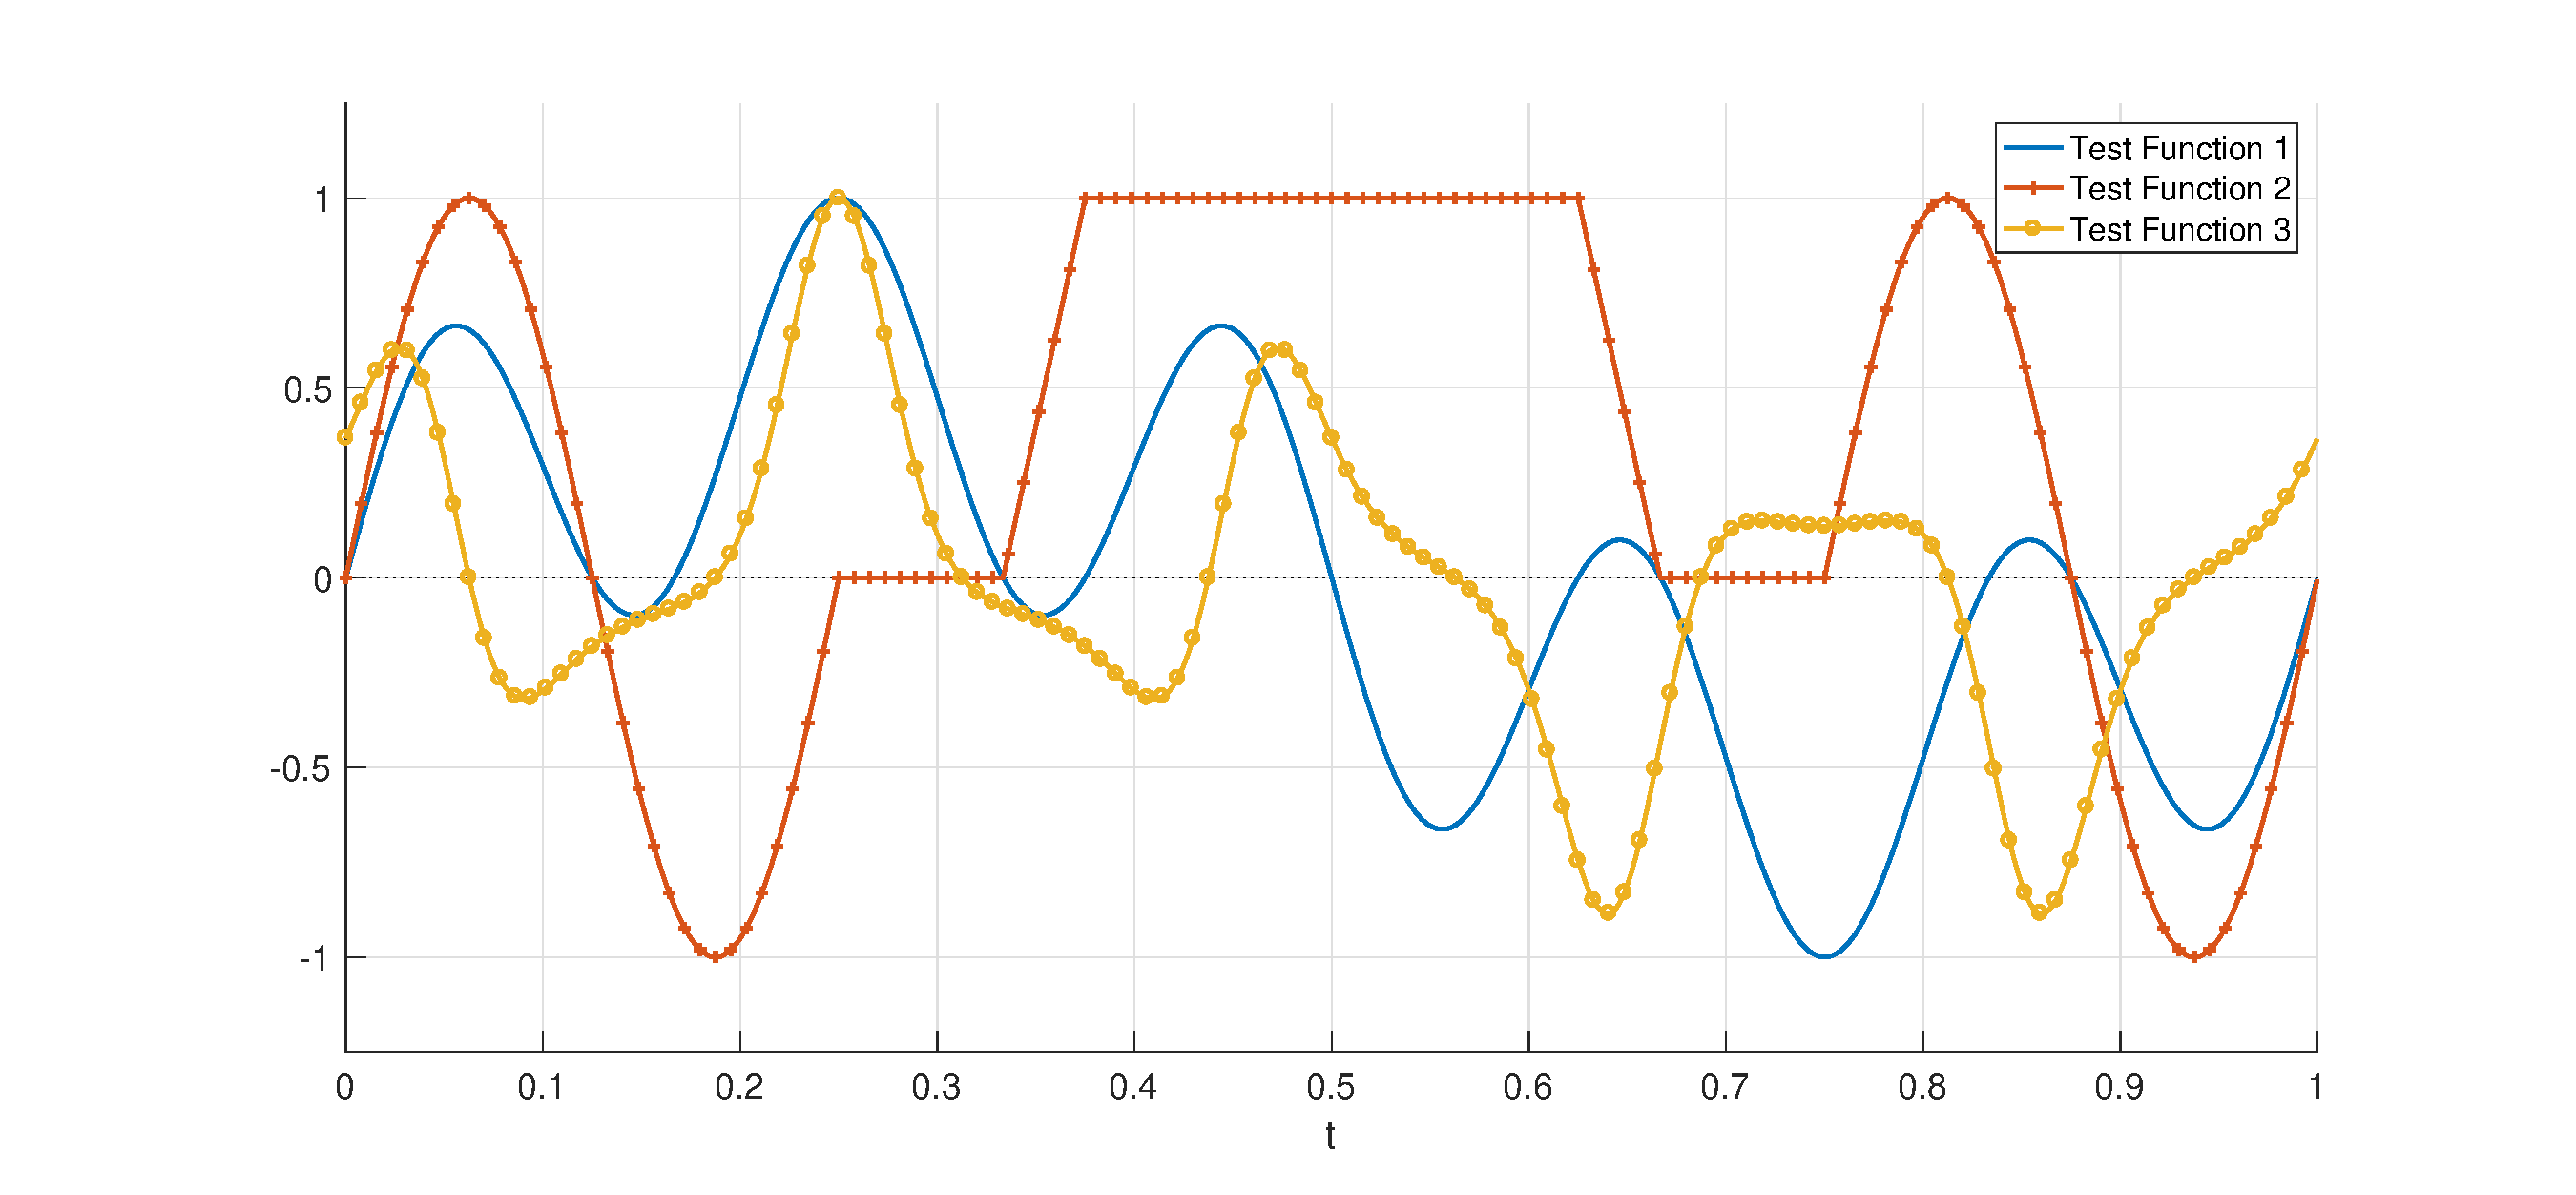
\includegraphics[scale = 0.45]{Figures/TestFunctions1D.eps}}
\caption{The three test functions considered in the numerical examples. Note that the second test function is only piecewise-smooth, while the first and second functions are smooth.}
\label{TestFunctions}
\end{figure}

The interval $[0,1]$ is discretized as equispaced points $0, 1/N, 2/N, \ldots, (N-1)/N$ for $N = 4096$. In other words, the interval is discretized as the vector $\tVec = [t_0,t_1,\ldots,t_{N-1}]$ with $t_\ell = \ell/N$. Samples of $g(x)$ are given at these points so that the discrete date $\gVec = [g_0,g_1,\ldots,g_{N-1}]$ has elements $g_\ell = g(t_\ell)$. The truncated Gaussian kernel $k(x,t)$ is assumed to be centered at the origin and compactly supported on the interval $[-\frac{1}{2},\frac{1}{2}]$. In the numerical examples, the width of the Gaussian kernels (i.e. the value of $1/2\noiseSD^2$ in \eqref{eq:Gaussian kernel}) is chosen to be 100 and 200. With a support of $[-\frac{1}{2},\frac{1}{2}]$, the test functions $f(t)$ must be defined on the interval $[-\frac{1}{2},\frac{3}{2}]$ for the convolution to be defined; see Chapter \ref{ch:Introduction}. As stated at the beginning of this chapter, $f(t)$ is initially defined over the interval $[0,1]$ and so the extensions of $f(t)$ on $[-\frac{1}{2},0)$ and $(1,\frac{3}{2}]$ will reflect the boundary condition being imposed.

%\begin{figure}
%	\centerline{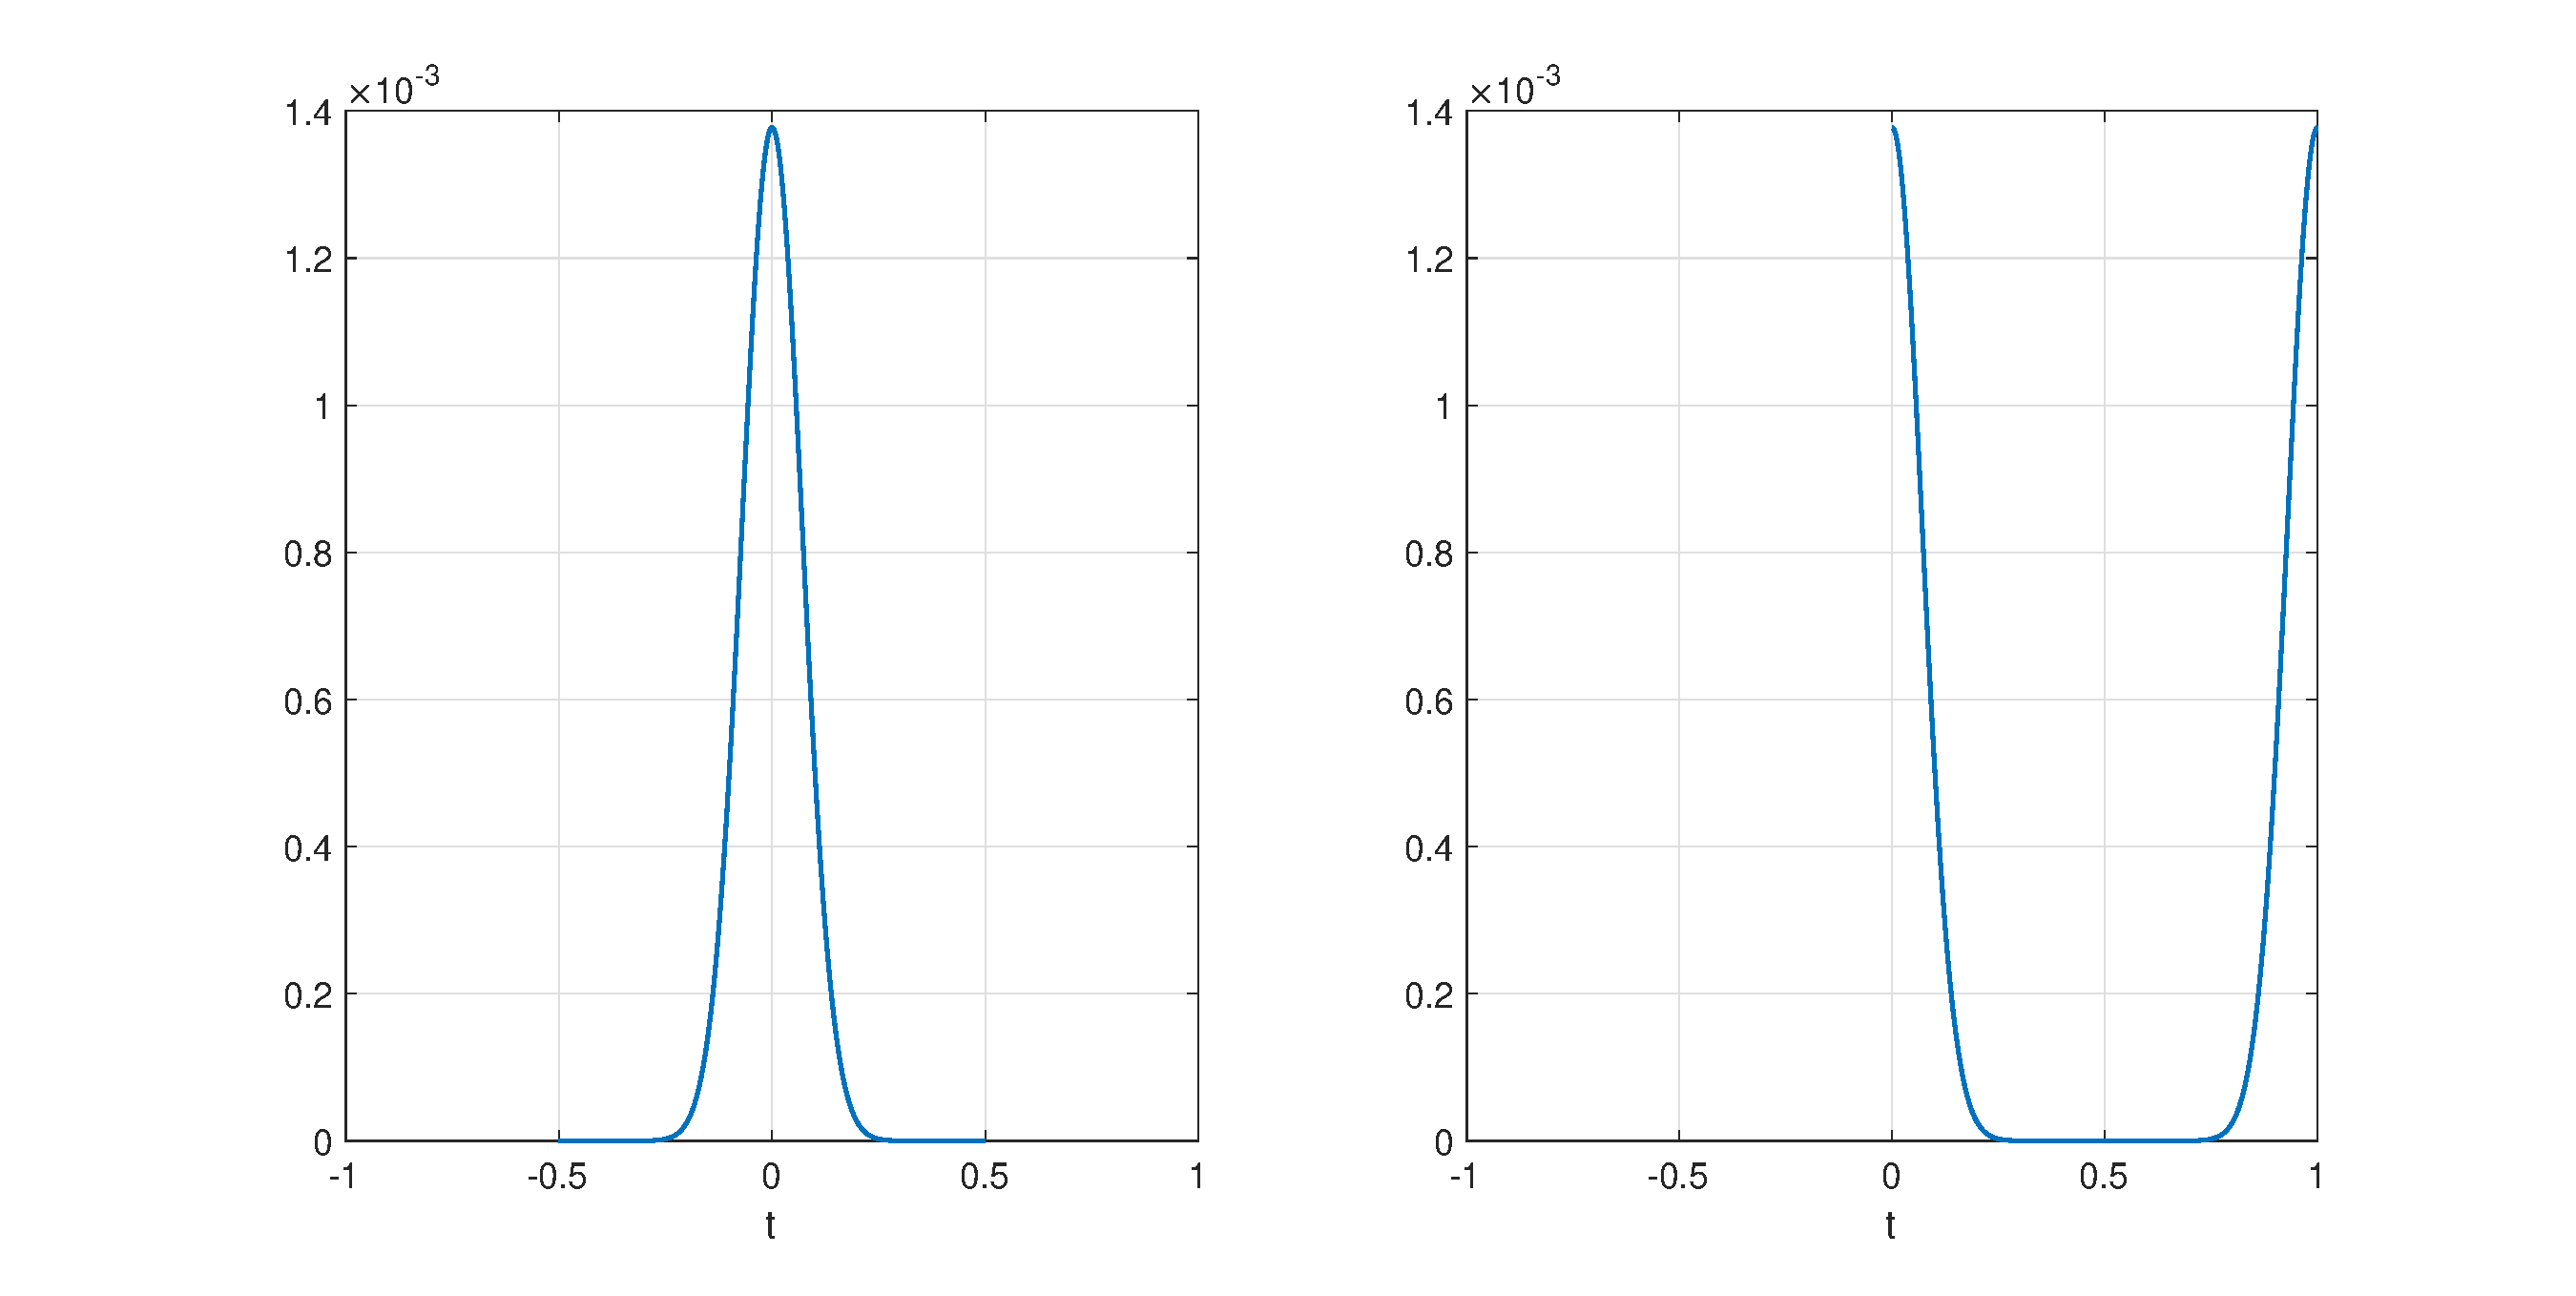
\includegraphics[scale = 0.45]{Figures/RegAndTroughGaussian.eps}}
%\caption{Plots of different discretizations of the kernel $k(t)$. The discretization on the left reflects the compact support of $k(t)$ on the interval $[-1/2,1/2]$. The discretization on the right represents the periodic extension of $k(t)$ on the interval $[0,1]$.}
%\label{RegAndTroughGaussian}
%\end{figure}

With the discretizations $\fVec$ and $\kVec$ determined, the discretization $\gVec$ of $g(t)$ can be evaluation using either a circular convolution or a linear convolution with appropriate vector padding. Ultimately the vectors $\fVec$, $\kVec$, and $\gVec$ are vector discretizations of $f(t)$, $k(x-t)$, and $g(t)$, respectively. \par
Overall, two selections for the width of the Gaussian kernel, two selections 5 and 25 for SNR value, and three test functions lead to a total of 12 configurations. For each configuration, 20 noise realizations were generated and tested. The full resolution problem was constructed using $N = 4096$ points. The downsamped resolutions were selected as $n \in \{16,32,\ldots,2048\}$ for a total of nine resolutions (eight values of $n$). \par 
A primary challenge of using the UPRE method with downsampled signals is that for a course downsampling (in other words, a small number of sample points), the resulting UPRE graphs are shallow. This shallowness makes finding a minimum difficult, and sometime the selected parameter is too small. Figure \ref{fig:UPRElambdas} shows that there are often outlier parameters that are too small, even sometimes for downsamplings with a moderate number of points. At $n = 16$, the range of the parameter values is larger than for the other downsampling levels, which can also be attributed to the shallowness of the function graphs. \par 
A consequence of choosing the regularization parameter to be too small is that the resulting relative errors are large; the outliers in Figure \ref{fig:UPREerrors} are the relative errors corresponding to the parameter outliers in Figure \ref{fig:UPRElambdas}. Unfortunately the error outliers can be significant, as even evidenced by the outlier at the full $N = 4096$ level. \par 
Fortunately, the averaged UPRE method appears to overcome the effects of the outliers. Figure \ref{fig:UPRElambdas} shows that for each downsampling level, the parameter found using the average UPRE method was larger than the mean of the parameters found by applying the UPRE to the noise realizations individually. As a result, the corresponding relative errors are less than the means of the errors for each downsampling level, displayed in Figure \ref{fig:UPREerrors}. However, the benefit derived from using the averaged UPRE method might be a consequence of the outliers themselves. Following the approximate region of the minimums of the UPRE functions (shown in Figure \ref{fig:UPREfunctions}), the functions increase rapidly. Thus functions that are excessively shallow may have this region of rapid increase located before the region of the minimums of the other functions. It could be the case that when the average UPRE function is formed, these outlier regions of rapid increase might push the final minimum toward a location that is actually beyond the region of the minimums of the non-outlier functions, resulting in a parameter that is larger than the mean of the individual parameters. Of course, this analysis is not rigorous and perhaps worthy of further investigation. 

\begin{figure}
	\centering
	\begin{subfigure}[b]{0.45\textwidth}
        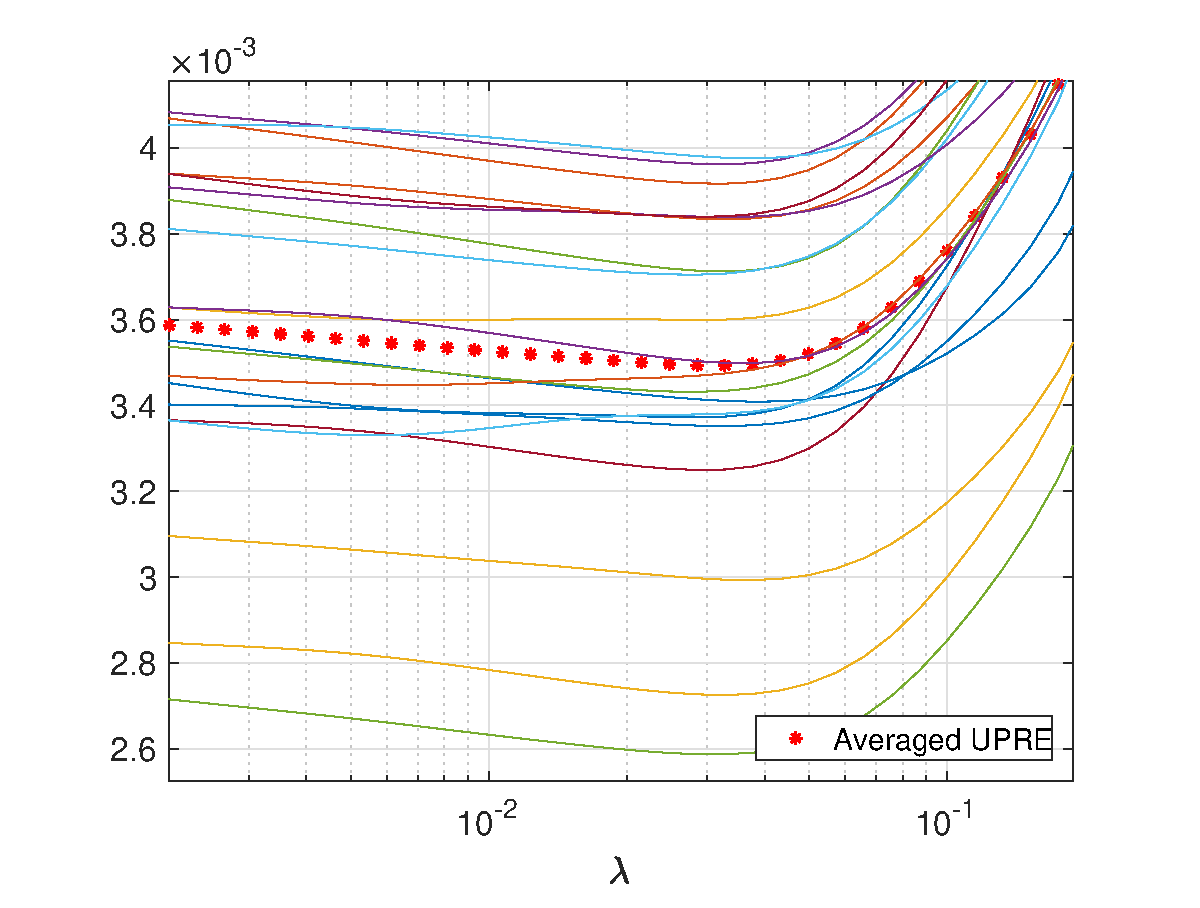
\includegraphics[width=\textwidth]{Figures/UPRE_AvgPlot1D_F1_S15_W100_R20.eps}
        \caption{}
        \label{fig:UPREfunctions}
    \end{subfigure}
    \begin{subfigure}[b]{0.45\textwidth}
        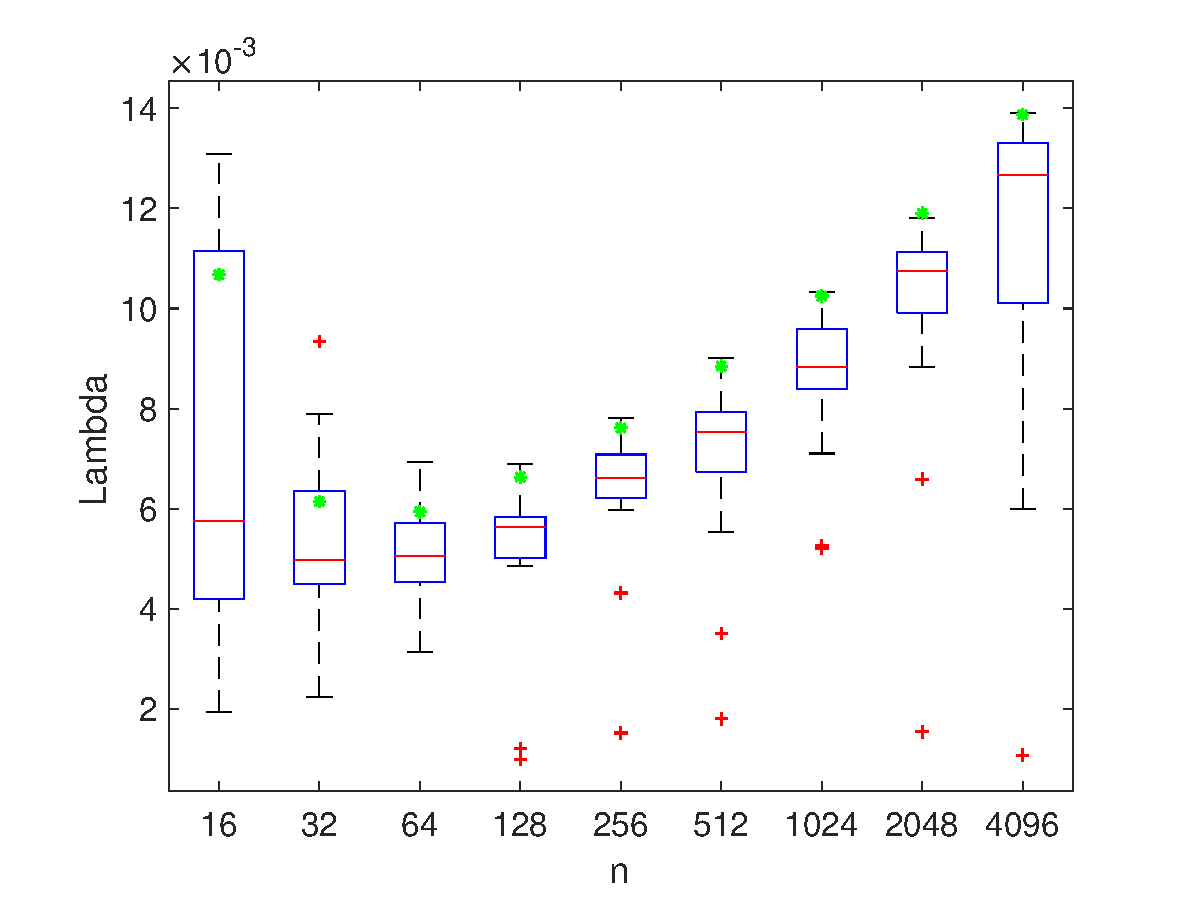
\includegraphics[width=\textwidth]{Figures/UPRE_LamPlot1D_F1_S15_W100_R20.eps}
        \caption{}
        \label{fig:UPRElambdas}
    \end{subfigure}
    \begin{subfigure}[b]{0.45\textwidth}
        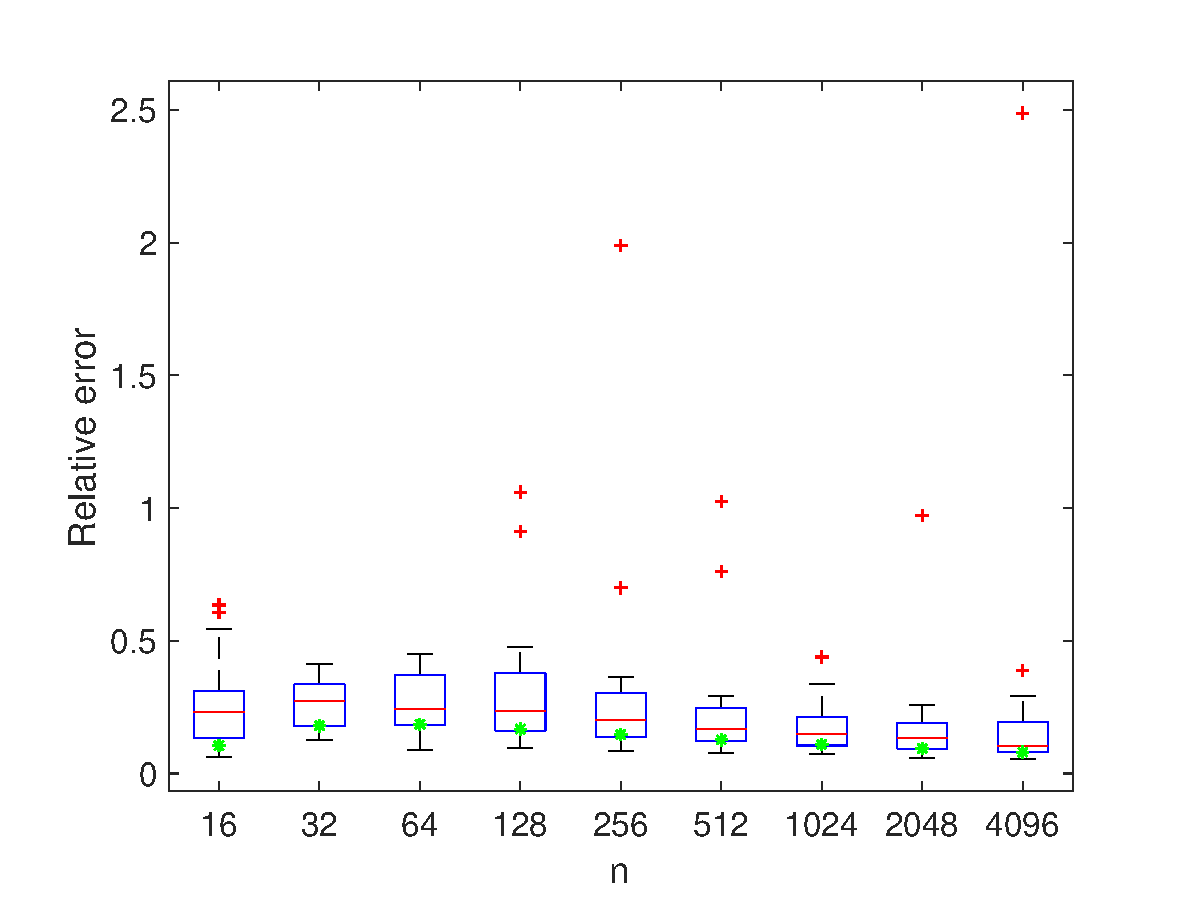
\includegraphics[width=\textwidth]{Figures/UPRE_ErrPlot1D_F1_S15_W100_R20.eps}
        \caption{}
        \label{fig:UPREerrors}
    \end{subfigure}
    \caption{Three plots showing the averaged UPRE results for the first test function with an SNR of 15 and  a Gaussian width parameter of 100. Figure \ref{fig:UPREfunctions} shows a zoomed-in portion of the averaged UPRE graph in comparison with graphs pertaining to the 20 noise realizations at a downsampling level of $n = 128$. Figure \ref{fig:UPRElambdas} shows that the resulting regularization parameter is typically greater than the average of the individual regularization parameters. Figure \ref{fig:UPREerrors} shows that the relative error corresponding to the parameter chosen from the average UPRE method is less than the average of the individual relative errors.}
\label{fig:UPREplots}
\end{figure} 

The numerical results of the GCV method are similar to those of the UPRE method. At times the graphs of the GCV functions are shallow and thus difficult to minimize. This is apparent from the parameter outliers in Figure \ref{fig:GCVlambdas} and the corresponding error outliers in Figure \ref{fig:GCVerrors}. The range of the parameters selected at the $n = 16$ is again significant. Some of the parameters at this level were selected so small (quite near to zero) so that the relative errors were excessively large; the largest relative error was approximately 35, and as a result the vertical axis in Figure \ref{fig:GCVerrors} had to be scaled so that errors larger than 2 are simply grouped in a non-scaled region to produce a tractable plot. \par 
In contrast to the UPRE method, the averaged version of the GCV method selected a regularization parameter that was worse than those selected by using individual noise realizations. The consequence of this is that the corresponding relative errors were larger than the mean of the individual relative errors. Thus the averaged GCV method does not appear to be a viable parameter selection approach.
%As previously mentioned, for the minimization-based methods UPRE and GCV, the shallowness of some of the curves made finding a meaningful minimum difficult. The approach that might be worth considering is to find the location of maximum curvature, which follows the observations and analysis presented in \cite{HansenOLeary}. \par 
%The signed curvature of a function $f$, assuming appropriate differentiablility, is
%\begin{equation}
%\kappa(x) = \frac{f''(x)}{(1+(f'(x))^2)^{3/2}}.
%\label{Eq:Curvature}
%\end{equation}
%Including the sign of the curvature is useful since a location of maximum curvature could be associated with local maximum instead of a minimum. A numerical approximation to \eqref{Eq:Curvature} can be readily obtained by discretizing $f$ on the domain of interest and using the finite difference approximations
%\[f'(x) \approx \frac{x_{j+1} - x_{j}}{\Delta{x}} \text{ and } f''(x) \approx \frac{x_{j-1} - 2x_j + x_{j+1}}{(\Delta{x})^2}\]
%for approximations of the derivatives. In MATLAB, the built-in function \texttt{diff} can be used to generate the derivative approximations. \par 
%Once a discretization of curvature is obtained, the location of maximum curvature is determined and this location is taken to be the regularization parameter from the UPRE and GCV methods. While the approach of maximizing curvature is not the same as finding a minimum a function itself, this approach could avoid the numerical challenges of minimizing the shallow UPRE and GCV functions. 

\begin{figure}
	\centering
	\begin{subfigure}[b]{0.45\textwidth}
        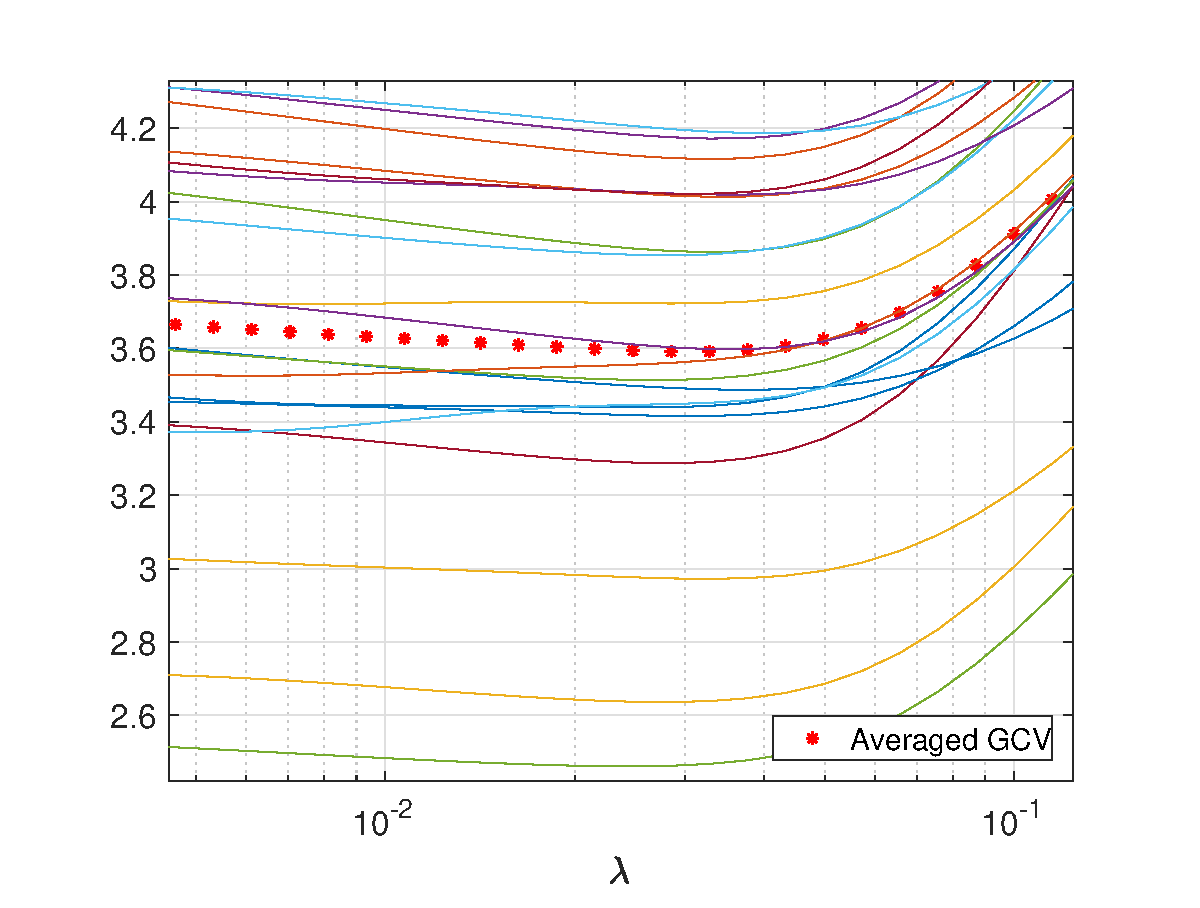
\includegraphics[width=\textwidth]{Figures/GCV_AvgPlot1D_F1_S15_W100_R20.eps}
        \caption{}
        \label{fig:GCVfunctions}
    \end{subfigure}
    \begin{subfigure}[b]{0.45\textwidth}
        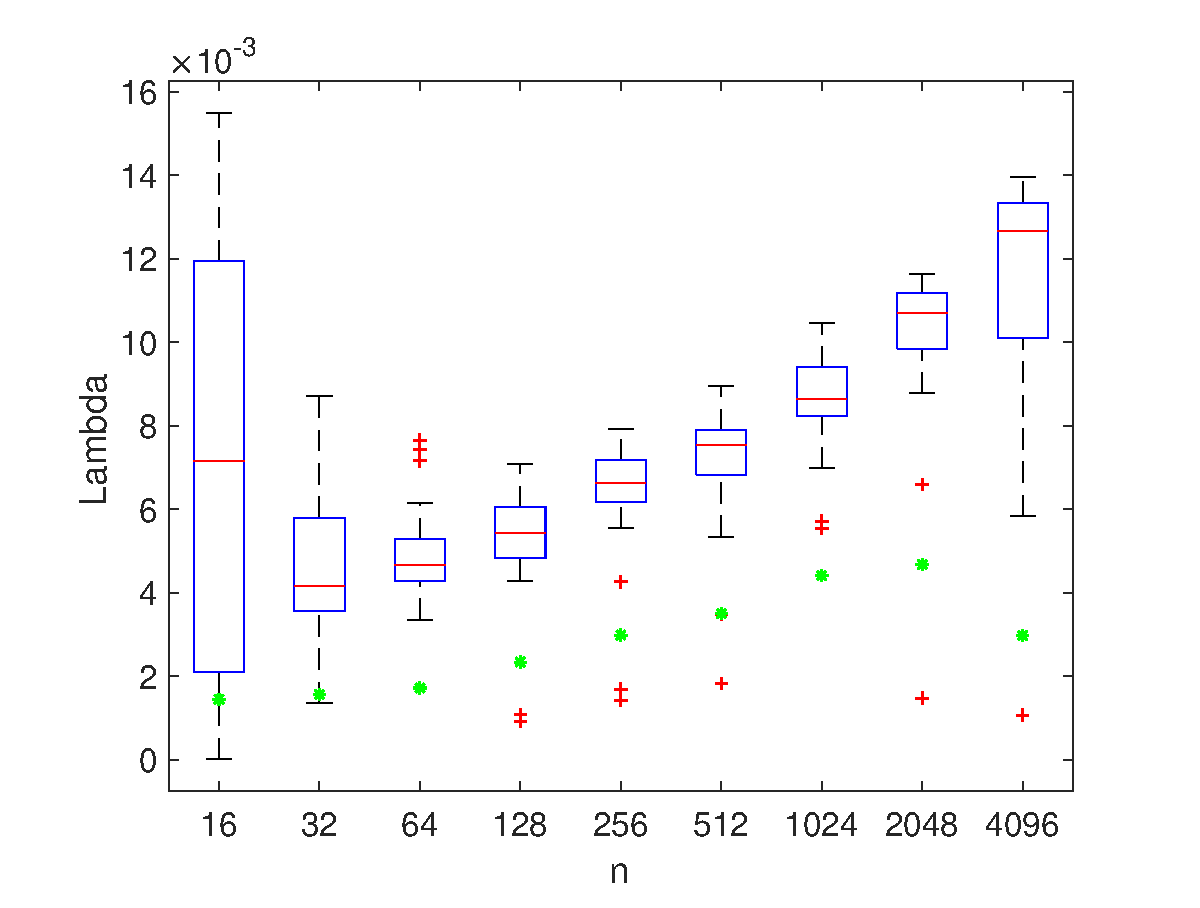
\includegraphics[width=\textwidth]{Figures/GCV_LamPlot1D_F1_S15_W100_R20.eps}
        \caption{}
        \label{fig:GCVlambdas}
    \end{subfigure}
    \begin{subfigure}[b]{0.45\textwidth}
        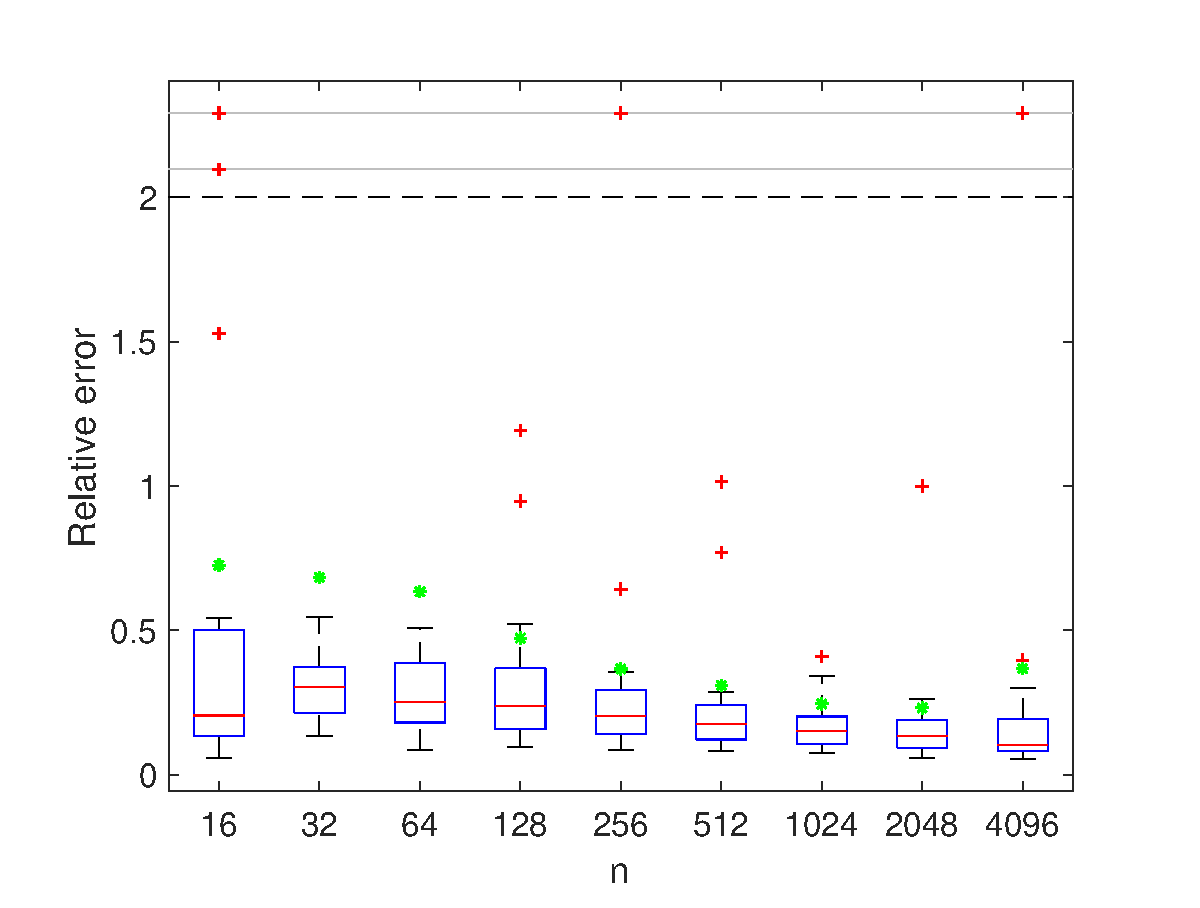
\includegraphics[width=\textwidth]{Figures/GCV_ErrPlot1D_F1_S15_W100_R20.eps}
        \caption{}
        \label{fig:GCVerrors}
    \end{subfigure}
    \caption{Three plots showing the averaged GCV results for the first test function with an SNR of 15 and a Gaussian width parameter of 100. Figure \ref{fig:GCVfunctions} shows a zoomed-in portion of the averaged GCV graph in comparison with graphs pertaining to the 20 noise realizations at a downsampling level of $n = 128$. Figure \ref{fig:GCVlambdas} shows that the resulting regularization parameter is typically less than the average of the individual regularization parameters. Figure \ref{fig:GCVerrors} shows that the relative error corresponding to the parameter chosen from the average GCV method is greater than the average of the individual relative errors.}
\label{fig:GCVplots}
\end{figure}

\chapter{The DCT approach} \label{ch:DCT}

The first boundary condition that will be considered is the Neumann boundary condition, defined by setting
\[\begin{cases}
f_{-1} = f_0 \\
f_{-2} = f_1 \\
\vdots \\
f_{-m+2} = f_{n-1}
\end{cases} ~ \text{and} ~
\begin{cases}
f_{n} = f_{n-1} \\
f_{n+1} = f_{n-2} \\
\vdots \\
f_{n+m-1} = f_{n-m}
\end{cases}.\]
Letting $J$ denote the $n \times n$ exchange matrix, the Neumann boundary condition allows for \eqref{eq: Tf = g} to be written as
\begin{equation}
\label{eq:Neumann Kf = g}
K\fVec = [(0~|~T_{l})J + T + (T_{r}~|~0)J]\fVec = \gVec,
\end{equation}
where $(0~|~T_{l})$ and $(T_{r}~|~0)$ are the $n \times n$ Toeplitz matrices formed by augmenting $T_{l}$ and $T_{r}$ with $n-m+1$ zero columns. As a result, the matrices $(0~|~T_{l})J$ and $(T_{r}~|~0)J$ are Hankel matrices. Therefore since $T$ is a Toeplitz matrix, the sum $[(0~|~T_{l})J + T + (T_{r}~|~0)J]$ is a Toeplitz-plus-Hankel matrix. Fortunately, this type of matrix is diagonalized by the DCT as stated in Section \ref{sec:Discrete trig. transforms}. The DCT-versions of the UPRE function \eqref{eq:UPRE DCT}, the GCV function \eqref{eq:GCV DCT}, and the discrepancy principle function \eqref{eq:DP DCT} can thus be used to select the Tikhonov regularization parameter $\regparam$. \par 
An version of the Downsampling Theorem can be obtained for the DCT. First, the following lemma will be established.
\begin{lemma}
Let $\mathbf{x} \in \mathbb{C}^N$, where $N = LM$ for positive integers $L$ and $M$. Then
\begin{align*}
\Re\left(\alias_L(\mathbf{x})\right) = \alias_L\left(\Re(\mathbf{x})\right), \\
\Im\left(\alias_L(\mathbf{x})\right) = \alias_L\left(\Im(\mathbf{x})\right).
\end{align*}
\end{lemma}
\begin{proof}
Let $\mathbf{a} = \Re(\alias_L(\mathbf{x}))$ and $\mathbf{b} = \alias_L(\Re(\mathbf{x}))$. By the definition of the aliasing operator and the linearity of taking the real part,
\[a_j = \Re\left(\sum_{k=0}^{L-1} x_{j+kM}\right) = \sum_{k=0}^{L-1} \Re(x_{j+kM}) = b_j.\]
The proof for the imaginary part is identical.
\end{proof}

A two-dimensional Fredholm integral equation of the first kind is
\begin{equation}
g(x,y) = \int_c^d \int_a^b k(x,y,s,t)f(s,t)~ds~dt.
\label{eq:FIE_2D}
\end{equation}
If the kernel satisfies $k(x,y,s,t) = k(x-s,y-t)$ and the limits of integration are infinite, then \eqref{eq:FIE_2D} represents two-dimensional convolution:
\begin{equation}
g(x,y) = \iint_{\mathbb{R}^2} k(x-s,y-t)f(s,t)~ds~dt.
\label{eq:Con_2D}
\end{equation}
Since an image can be considered a function $f : \mathbb{R}^2 \rightarrow \mathbb{R}$, the process of finding solutions to equations of the form \eqref{eq:Con_2D} is commonly referred to \textit{image deblurring}. For an extensive handling of image deblurring techniques, see \cite{HansenNagyOLeary} and \cite[Ch.~5]{Vogel:2002}. \par
If the support of $k(x-s,y-t)$ is $[a_k,b_k] \times [c_k,d_k]$ and information about $g(x,y)$ is known only in $[a_g,b_g] \times [c_g,d_g]$, then the integral equations for the values of $g(x,y)$ on the vertices of the rectangles are
\begin{align*}
g(a_g,c_g) &= \int_{c_g-d_k}^{c_g-c_k} \int_{a_g-b_k}^{a_g-a_k} k(a_g-s,c_g-t)f(s,t)~ds~dt \\
g(b_g,c_g) &= \int_{c_g-d_k}^{c_g-c_k} \int_{b_g-b_k}^{b_g-a_k} k(b_g-s,c_g-t)f(s,t)~ds~dt \\
g(b_g,d_g) &= \int_{d_g-d_k}^{d_g-c_k} \int_{b_g-b_k}^{b_g-a_k} k(b_g-s,d_g-t)f(s,t)~ds~dt \\
g(a_g,d_g) &= \int_{d_g-d_k}^{d_g-c_k} \int_{a_g-b_k}^{a_g-a_k} k(a_g-s,d_g-t)f(s,t)~ds~dt.
\end{align*}
For the sake of simplicity, assume that the support of $k(x-s,y-t)$ is $[-\frac{1}{2},\frac{1}{2}] \times [-\frac{1}{2},\frac{1}{2}]$ and information about $g(x,y)$ is known only in the unit square $[0,1] \times [0,1]$. Then
\begin{align*}
g(0,0) &= \int_{-\frac{1}{2}}^{\frac{1}{2}} \int_{-\frac{1}{2}}^{\frac{1}{2}} k(-s,-t)f(s,t)~ds~dt \\
g(1,0) &= \int_{-\frac{1}{2}}^{\frac{1}{2}} \int_{\frac{1}{2}}^{\frac{3}{2}} k(1-s,-t)f(s,t)~ds~dt \\
g(1,1) &= \int_{\frac{1}{2}}^{\frac{3}{2}} \int_{\frac{1}{2}}^{\frac{3}{2}} k(1-s,1-t)f(s,t)~ds~dt \\
g(0,1) &= \int_{\frac{1}{2}}^{\frac{3}{2}} \int_{-\frac{1}{2}}^{\frac{1}{2}} k(-s,1-t)f(s,t)~ds~dt.
\end{align*}
From these equations, the domain of definition of $f(s,t)$ needed for the existence of the integrals is $[-\frac{1}{2},\frac{3}{2}] \times [-\frac{1}{2},\frac{3}{2}]$. Thus if information about $f(s,t)$ is only required in $[0,1] \times [0,1]$, boundary conditions must be imposed.

%\section{Resolution Analysis} \label{ch:Resolution Analysis}
%Our goal is to determine the efficacy of downsampling for regularization parameter estimation, the effects of downsampling on the parameter estimation methods must be carefully examined. The parameter estimation methods are considered from the perspective of the DFT, and so downsampling must be viewed from the same perspective. \par 
%One of the most powerful results pertaining to sampling a signal for use in Fourier analysis is the Shannon-Whittaker Sampling Theorem, which is given here without proof. The version of the theorem pertains to the Fourier transform, defined for a function $f \in L^1(\mathbb{R})$ by
%\begin{equation}
%\dft{f}(\omega) = \frac{1}{\sqrt{2\pi}}\int_{-\infty}^{\infty} f(t)\exp(-i\omega{t})\: dt. 
%\label{eq:FourierTransform}
%\end{equation}
%The variable $\omega$ represents frequency. 
%\begin{SWST}
%Suppose that $\dft{f}(\omega)$ is continuous, piecewise smooth, and $\dft{f}(\omega) = 0$ for $|\omega| > \Omega$, where $\Omega$ is some fixed, positive frequency. Then $f = \mathcal{F}^{-1}(\dft{f})$ is completely determined by its values at the points $t_j = j\pi/\Omega$ for $j = 0,\pm 1,\pm 2,\ldots$. More precisely, $f$ has the series expansion
%\[f(t) = \sum_{j=-\infty}^{\infty} f\left(\frac{j\pi}{\Omega}\right)\frac{\sin(\Omega{t}-j\pi)}{\Omega{t}-j\pi},\]
%which converges uniformly. 
%\end{SWST}
%Given the smallest frequency $\Omega$ such that $\dft{f}(\omega) = 0$ for $|\omega| > \Omega$, the quantity $\Omega/2\pi$ is called the \textit{Nyquist frequency} and the quantity $\Omega/\pi$ is called the \textit{Nyquist rate}. Functions for which $\Omega$ exists such that $\dft{f}(\omega) = 0$ for $|\omega| > \Omega$ are called \textit{band-limited}. \par 
%The test function $f(x) = \cos(4\pi{t})\sin(6\pi{t})$ is band-limited. Applying a product-to-sum identity allows for the function to be rewritten as
%\begin{equation}
%f(t) = \cos(4\pi{t})\sin(6\pi{t}) = \frac{1}{2}\left[\sin(10\pi{t}) + \sin(2\pi{t})\right].
%\label{eq:Test Function 1}
%\end{equation}
%Though $f$ is not in $L^1(\mathbb{R})$, its Fourier transform can be express using the Dirac delta function:
%\begin{equation}
%\dft{f}(\omega) = i\frac{\sqrt{\pi}}{2\sqrt{2}}\left[\delta(\omega - 10\pi) +\delta(\omega - 2\pi) - \delta(\omega + 2\pi) - \delta(\omega + 10\pi)\right].
%\label{eq:Test Function 1 FT}
%\end{equation}
%It is now clear from \eqref{eq:Test Function 1 FT} that $f$ is indeed band-limited because $\dft{f}(\omega) = 0$ for $|\omega| > 10$. The Sampling Theorem then states that $f$ must be sampled at greater than 20 equispaced points per unit interval for exact reconstruction. If the number of sample points is selected as a power of 2 (which is advantageous for computation of DFT's), then sampling $f$ at $2^5 = 32$ points would be ideal; a smaller power, such as $2^4 = 16$, would be insufficient in that the reconstruction would suffer from the effects of aliasing. \par 
%In contrast, the second test function \eqref{eq:Test Function 2} is not band-limited. This can be seen by computing the Fourier transform of the piece of $f$ on $[3/8,5/8]$:
%\begin{equation} 
%\int_{3/8}^{5/8} \exp(-i\omega{t}) \: dt = \frac{2\exp(-i\omega/2)\sin(\omega/8)}{\omega}.
%\label{eq:Test Function 2 FT}
%\end{equation}
%Certainly there does not exist an $\Omega > 0$ such that the expression in \eqref{eq:Test Function 2 FT} is zero for all $|\omega| > \Omega$.
